\documentclass[12pt, a4paper]{article}

\usepackage[utf8]{inputenc}
\usepackage[russian]{babel}
\usepackage{geometry}
\usepackage{mathtools}
\usepackage{verbatim}
\usepackage{indentfirst}
\usepackage{caption}
\usepackage{subcaption}
\usepackage{import}
\usepackage{xifthen}
\usepackage{pdfpages}
\usepackage{transparent}
\usepackage{graphicx}
\usepackage{caption}
\usepackage{hyperref}
\usepackage{float}

\newcommand{\norm}[1]{\lVert #1 \rVert}
\newcommand{\abs}[1]{\lvert #1 \rvert}
\usepackage[oglav,spisok,boldsect,eqwhole,figwhole,hyperref,hyperprint,remarks,greekit]{./style/fn2kursstyle}

\graphicspath{{./style/}{./figures/}}

\frenchspacing

\title{Итерационные метды решения систем линейных алгебраических уравнений}
\lab{2}
\author{М.\,А.~Каган}
\creator{И.\,А.~Яковлев}
\supervisor{}
\group{ФН2-51Б}
\date{2024}

\begin{document}
	\maketitle
	\tableofcontents
	
	\newpage
	
	\section{Исходные данные}
	
	Система линейных уравнений №1:
	\[
	\left \{ \begin{array}{ccccccccc}
		0.2910 x_1  & +   &   1.8100 x_2 & +   &     9.3110 x_3 & +    &    9.1100 x_4 & = & 4.2280\\
		1.4500  x_1 & + &     8.5790 x_2 & +  &     44.1950 x_3  & +  &    42.9950 x_4  & = & 20.4290\\
		-0.2900 x_1  & - &     1.7980 x_2 & - &      9.2500 x_3   & - &    9.0500 x_4 & = & -4.2080  \\
		0.0000  x_1  & + &     0.0820 x_2  & +  &     0.4100 x_3 & +  &      0.4500 x_4 & = & 0.1220
	\end{array}	\right.
	\]
	 
	Система линейных уравнений №2:
	 \[
	 \left \{ \begin{array}{ccccccccc}
	 -106.4000 x_1 & - & 7.0000 x_2 & - & 4.9900 x_3 & + & 0.2600 x_4 & = & 1040.8100\\
	3.6100 x_1 & + & 22.2000 x_2 & - & 8.5900 x_3 & - & 8.9200 x_4 & = & 615.4100 \\
	 2.2800 x_1 & + & 7.7500 x_2 & + & 52.2000 x_3 & + & 9.6500 x_4 & = & 427.5400 \\
	 -9.0000 x_1 & + & 5.8100 x_2 & - & 0.0900 x_3 & + & 136.8000 x_4 & = & -265.3500
	\end{array}	\right.
	 \]  
	\section{Краткие сведения}
	Пусть $A$ --- невырожденная матрица $n \times n$, $b$ --- ненулевой n-мерный вектор. Необходимо найти такой n-мерный вектор $x$, чтобы он удовлетворял уравнению
	\begin{equation}
		\label{eq}
		A x = b.
	\end{equation}
  
	\subsection{Метод простой итерации}
\textbf{Методом простой итерации} называется явный метод
$$
\frac{x^{k+1} - x^k}{\tau} + Ax^k = b, \quad k = 0, \, 1, \, 2, \dots.
$$
Здесь $\tau$ ---  специально выбираемый итерационный параметр.
	\subsection{Метод Якоби}
	
	Метод Якоби заключается в том, чтобы рассматривать матрицу $A$ как сумму $A_1 + D + A_2$, где $D$ матрица с элементами на главной диагонали, совпадающей с элементами главной диагонали $A$, $A_1$ матрица с элементами под главной диагональю совпадающей с элементами под главной диагональю матрицы $A$. Общий вид итерационной схемы:
	\[
	D x^{k+1} = f - A_1 x^k - A_2 x^k. 
	\]
			
	\subsection{Метод релаксации}	

	Метод релаксации является обобщением метода Зейделя: добавляется итерационный параметр $\omega$.
	Общий вид итерационной схемы:
	\[
	(E + \omega D^{-1} A_1) x^{k+1} = ((1-\omega)E - \omega D^{-1}A_2) x^{k} + \omega D^{-1}b.
	\]
	


	\subsection{Метод Зейделя}
Метод Зейделя является частным случаем \textbf{метода релаксации} с $\omega = 1$. Каноническая форма \textbf{метода Зейделя} имеет вид
$$
\left( D + L \right ) \left( x^{k+1} - x^k \right ) + Ax^k = b, \quad k = 0, \, 1, \, 2, \dots.
$$

	% \section{Ход работы}
	% \subsection{Исходные данные}
	% \subsection{Результаты расчетов}
	% \subsection{Анализ результатов}
	
	\section-{Контрольные вопросы}
	\begin{enumerate}
		\item \textbf{Почему условие $\norm{C} < 1$ гарантирует сходимость итерационных методов?}
		
		\vspace*{0.2cm}
		\textit{\textbf{Ответ:}}
	
Условие $\norm{C} < 1$ связано с тем, что для нахождения единственного решения (единственной неподвижной точки) оператору $C$ необходимо быть сжимающим, а из определения сжимающего оператора следует, что его норма должна быть строго меньше единицы.

		\textbf{\item Каким следует выбирать итерационный параметр $\tau$ в методе простой итерации для увеличения скорости сходимости? Как выбрать начальное приближение $x_0$?}
		 
		\vspace*{0.2cm}
		\textit{\textbf{Ответ:}}
		
		В общем виде последовательность приближений методом простой итерации задается следующей рекуррентной формулой:
		\begin{equation}
			\label{eq:рекурентная-формула-КВ}
			x^{k+1} = (E - \tau A)x^{k} - \tau f.
		\end{equation}
		Если принять во внимание равенство
		\[
		x = (E - \tau A)x - \tau f.
		\]
		и вычесть его из формулы (\ref{eq:рекурентная-формула-КВ}) тогда будет верна оценка
		\[
		\norm{x^{k+1} - x} \le \norm{E - \tau A} \, \norm{x^{k} - x}.
		\]
		Поскольку неравенство верно для любого $k$:
		\[
		\norm{x^{k+1} - x} \le \norm{E - \tau A}^2 \, \norm{x^{k-1} - x} \le \ldots \le \norm{E - \tau A}^{k+1} \, \norm{x^0 - x}
		\]
		Таким образом, чтобы увеличить скорость сходимости, необходимо выбрать $\tau$ и $x^0$ таким образом, чтобы $\norm{E - \tau A}$ и $\norm{x^0 - x}$ были минимальны. Однако, поскольку $x$ неизвестна заранее, можно найти нижнюю оценку из неравенства
		\[
		\norm{A x^0 - A x} \norm{A}^{-1}  = \norm{A(x^0 - x)} \norm{A}^{-1} \le \norm{x^0 - x}
		\] 

		Если матрица $A$ симметричная и положительно определенная, то оптимальным параметр $\tau = \sfrac{2}{\lambda_{min}+\lambda_{max}}$, где $\lambda_{min},\;\lambda_{max}$ минимальный и максимальный собственные значения матрицы $A$.
			
		\textbf{\item На примере системы из двух уравнений с двумя неизвестными дайте геометрическую интерпретацию метода Якоби, метода Зейделя, метода релаксации.}
		
		\vspace*{0.2cm}
		\textit{\textbf{Ответ:}}

Решения системы двух линейных уравнений можно интерпретировать как задачу поиска пересечения двух прямых на плоскости.

Рассмотрим метод Якоби. В этом случае итерационный процесс организуется следующим образом:
\begin{equation*}
        	\begin{cases}
        		a_{11} x^{k+1}_1 + a_{12} x^k_2 = f_1,\\
        		a_{21} x^{k}_1 + a_{22} x^{k+1}_2 = f_2.\\
        	\end{cases}
\end{equation*}
Каждое из уравнений задает некоторую прямую, точное решение $\hat{x}$ лежит на их пересечении. Приведем картинку с поэтапным поиском приближений \mbox{(рис. 1, \emph{a})}:
	\begin{figure}[H]
			\centering
			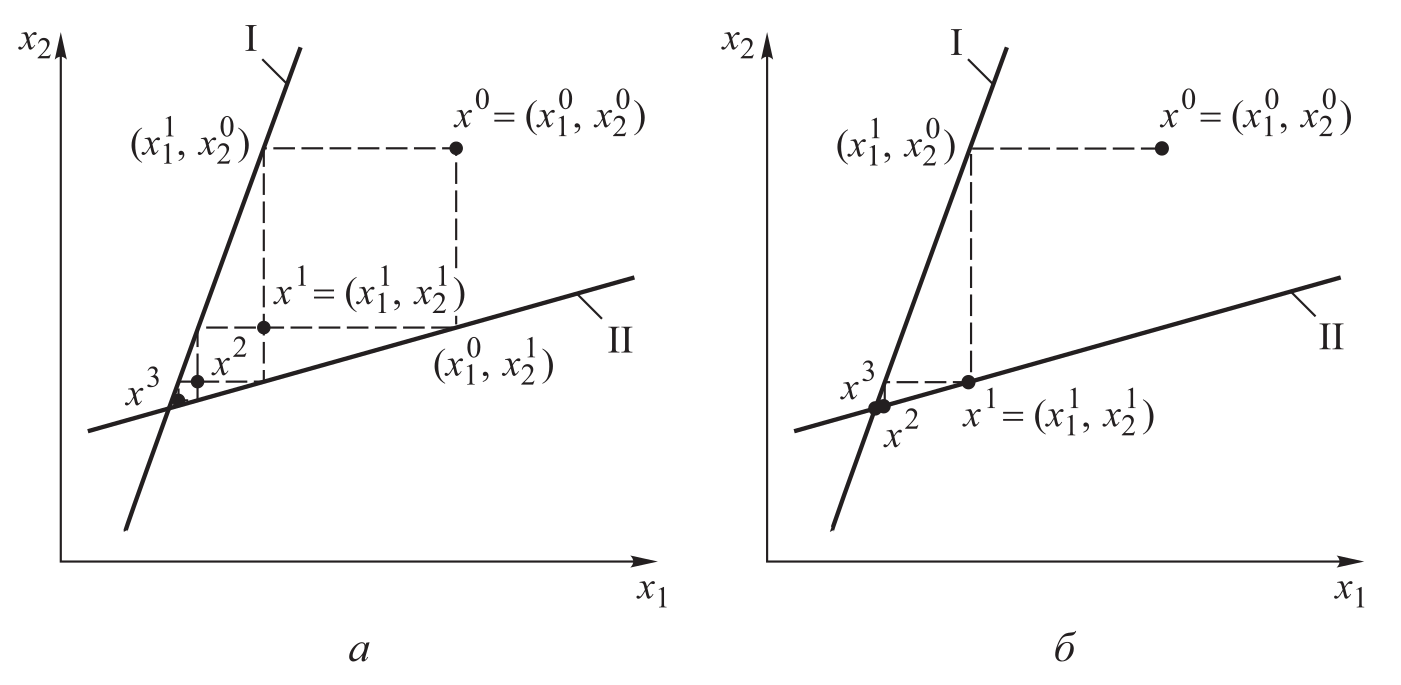
\includegraphics[width=0.8\linewidth]{geom_yak_zeyd.png}
			\caption{Геометрическая интерпретация метода Якобки (а) и Зейделя (б)}
			\label{yakzeyd}
	\end{figure}
Можно отметить, что в отличие от метода Зейделя (рис. 1, \emph{б}), ни одно из приближений $x^K$ не лежит на прямых I и II, т.е. ни для одного из уравнений невязка не обращается в нуль.

Итерационный процесс метода Зейделя задается следующим образом:
\begin{equation*}
        	\begin{cases}
        		a_{11} x^{k+1}_1 + a_{12} x^k_2 = f_1,\\
        		a_{21} x^{k+1}_1 + a_{22} x^{k+1}_2 = f_2.\\
        	\end{cases}
\end{equation*}
Здесь второе уравнение решено всегда точно.

При решении СЛАУ \emph{методом релаксации} следующее приближение осуществляется по формулам:
\begin{equation*}
        	\begin{cases}
        		a_{11} \left( x^{k+1}_1 - x^k_1 \right) = \omega \left( -a_{11} x_1^k - a_{12} x_2^k + f_1 \right),\\
        		a_{22} \left( x^{k+1}_2 - x^k_2 \right) = \omega \left( -a_{21} x_1^k - a_{22} x_2^k + f_2 \right).\\
        	\end{cases}
\end{equation*}
Смещение вдоль абсцисс определяется величиной:
\begin{equation*}
\abs{x^{k+1}_1 - x^k_1} = \frac{\omega}{\abs{a_{11}}} \cdot \abs{-a_{11} x_1^k - a_{12} x_2^k + f_1} = \omega \dfrac{d_1}{\abs{a_{11}} / \norm{\overrightarrow{l_1}}} = \omega \dfrac{d_1}{\abs{\cos \beta_1}},
\end{equation*}
где $d_1$ --- расстояние от точки $\left( x_1^k, \, x_2^k \right) $ до прямой I; $\overrightarrow{l_1} = (a_{11}, \, -a_{12} )$ --- направляющий вектор прямой I, $\beta_1$ --- угол между прямой I и осью ординат \mbox{(рис. 2, \emph{а})}.
\begin{figure}[H]
		\centering
		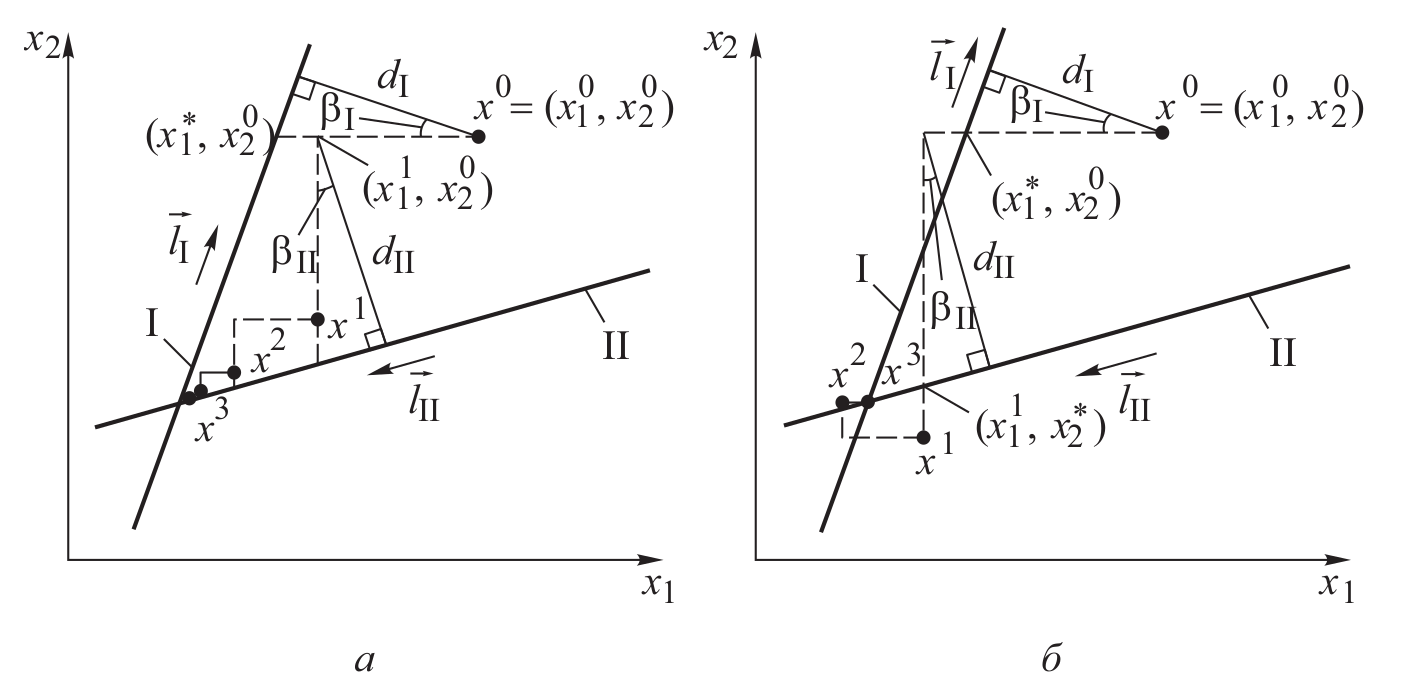
\includegraphics[width=0.8\linewidth]{geom_relax.png}
		\caption{Геометрическая интерпретация метода релаксации при $w < 1$ (\emph{а}) и $w > 1$ (\emph{б})}
		\label{relax}
\end{figure}
Таким образом, $\abs{x^{k+1}_1 - x^k_1} = \omega \abs{x^{*}_1 - x^k_1}$, где $x^*_1$ такой, что $a_{11} x^{k+1}_1 + a_{12} x^k_2 = f_1$. При $\omega < 1$ точки $\left( x_1^k, \, x_2^k \right), \left( x_1^{k+1}, \, x_2^k \right)$ находятся в одной полуплоскости относительно прямой I, а при $\omega < 1$ --- в разных полуплоскостях \mbox{(рис. 2, \emph{б}).} 

Если решать систему \emph{методом простой итерации}, то вычисления проводятся по формулам 
\begin{equation*}
\frac{x^{k+1} - x^k}{\tau} + Ax^k = f,
\end{equation*}
которые можно записать в виде
\begin{equation*}
        	\begin{cases}
		 x^{k+1}_1 - x^k_1 = \tau \left( -a_{11} x_1^k - a_{12} x_2^k + f_1 \right),\\
        		 x^{k+1}_2 - x^k_2 = \tau \left( -a_{21} x_1^k - a_{22} x_2^k + f_2 \right).\\
        	\end{cases}
\end{equation*}
Смещение вдоль оси абсцисс определяется величиной $\tau \abs{-a_{11} x_1^k - a_{12} x_2^k + f_1} = \tau d_{\text{I}} \norm{\overrightarrow{l_1}}$, вдоль оси ординат $\tau d_{\text{II}} \norm{\overrightarrow{l_{\text{II}} } }$ \mbox{(рис. 3)}.
\begin{figure}[H]
		\centering
		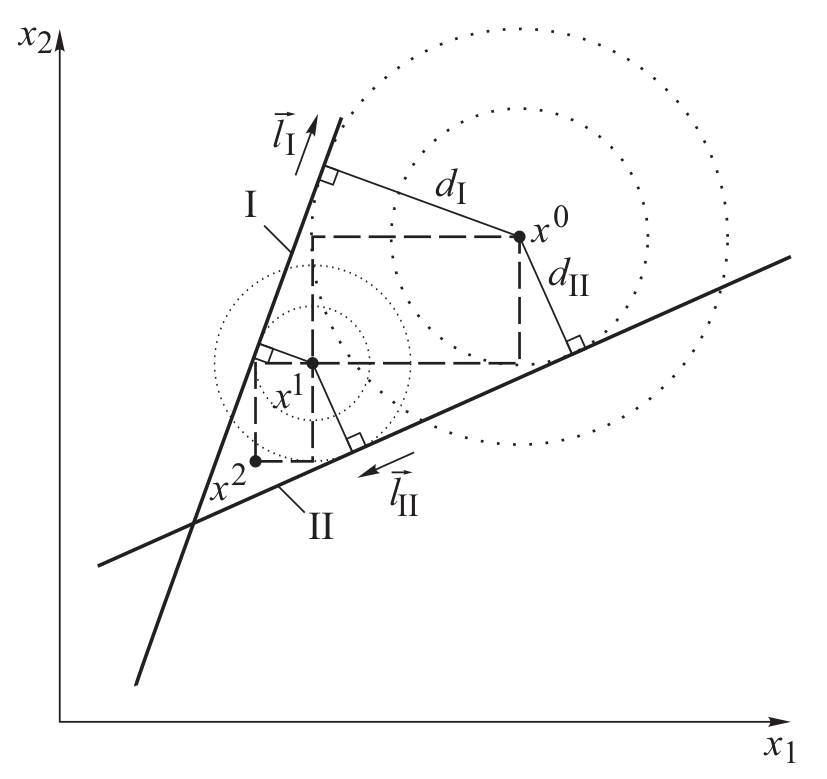
\includegraphics[width=0.45\linewidth]{geom_simple.png}
		\caption{Геометрическая интерпретация метода простой итерации при $\tau = 1$}
		\label{simple}
\end{figure}

		\textbf{\item При каких условиях сходятся метод простой итерации, метод Якоби, метод Зейделя и метод релаксации? Какую матрицу называют положительно определенной?}
		
		\vspace*{0.2cm}
		\textit{\textbf{Ответ:}}
		Рассмотрим итерационный процесс
		\begin{gather}
			x^{k+1} = C x^k + y, \; \text{где} \notag \\
			C = E - \tau B^{-1}; \; y = \tau B^{-1}f \notag
		\end{gather}
		сходится к решению системы $A x = f$ при любом начальном приближении $x^0$, тогда и только тогда, когда когда спектральный радиус матрицы перехода между итерации $\rho(C) < 1$.
		
		Если $A$ симметричная и положительно определенная, то метод сходится, то стационарный метод сходится если:
		\[
		B - 0.5 \tau A > 0
		\]
		\begin{enumerate}
			\item Из неравенства (\ref{eq:рекурентная-формула-КВ}) следует условие сходимости метода простой итерации: норма $\norm{E - \tau A}$ обязана быть меньше единицы. Заметим, что $\tau$ не нулевое.
			
			Если $A$ симметричная и положительно определенная, то метод сходится, если $\tau < 2/\lambda_{max}$.
			
			
			\item Рассмотрим рекуррентную формулу задающую последовательность приближений в методе Якоби:
			\begin{equation}
				\label{eq:рекурентная-формула-якоби-КВ}
				x^{k+1} = D^{-1}(f - A_1 x^k - A_2 x^k ). 
			\end{equation}
			Учитывая равенство
			\[
			x = D^{-1}(f - A_1 x - A_2 x ) 
			\]
			запишем оценку:
			\[
			\norm{x^{k+1} - x} \le  \norm{D^{-1} \bigl(A_1 + A_2\bigr)} \, \norm{x^k - x} \le \ldots \le  \bigl(\norm{D^{-1}\bigl( A_1 + A_2\bigr)}\bigr)^{k+1} \, \norm{x^0 - x}
			\]
			Таким образом для сходимости метода Якоби необходимо, чтобы
			  \[
			  	\norm{D^{-1} \bigl(A_1 + A_2\bigr)} \le 1.
			  \]
			Рассмотрим матрицу $С = D^{-1} \bigl(A_1 + A_2\bigr)$: его элементы будут удовлетворять условию:
			\[
			\begin{cases}
			c_{i \, j} = a_{i \, j} / d_{i \, i}, & \text{где} \; i \neq j; \\
			c_{i \, i} = 0.
			\end{cases}
			\]
			
			Докажем достаточность требования диагонального преобладания матрицы $A$: если доказать это утверждение для строчной нормы, то из равносильности сходимости эквивалентных норм будет следовать сходимость последовательности $\{x^k\}$ для любой нормы в конечномерном пространстве.
			
			Предположим, что $A$ обладает строгим диагональным преобладанием:
			\begin{equation}
				\label{ddd}
				|d_{i \, i}| = |a_{i \, i}| > \sum_{j=1, \, i \neq j}|a_{i \, j}|, \; \text{где} \; i = 1,\ldots,n.
			\end{equation}
			Рассмотрим норму $C$:
			\[
			\norm{C}_\infty = \max_{1\le i\le n}\sum_{j=1, \, i \neq j}^{n} |a_{i \, j} / d_{i \, i}|.
			\]
			Из неравенства (\ref{ddd}) следует, что норма $\norm{C}_\infty < 1$, следовательно метод Якоби сходится.
			
			В случае, если $A$ симметричная и положительно определенная, для сходимости метода должно выполнятся неравенство:
			\[
				D - 0.5 A > 0
			\]
			\item Рассмотрим оценку верную для последовательности приближений в методе релаксации:
			\begin{equation}
				\label{eq:рекурентная-формула-релаксация-КВ}
				\norm{x^{k+1} - x} \le \norm{C}\norm{x^{k} - x} \le \ldots \le \norm{C}^{k+1} \norm{x^{0} - x}. 
			\end{equation}
			 где $C = (E + \omega D ^{-1}A_1)^{-1} ((1-\omega)E - \omega D ^{-1}A_2)$. Таким образом метод релаксации сходится, если $\norm{C}< 1$. Заметим, что метод Зейделя частный случай метода релаксации при $\omega$ равной единице.
			 
			 В случае, если $A$ симметричная и положительно определенная $\omega $ должна лежать на отрезке $(0;2)$, это следует из неравенства:
			 \[
			 (D - \omega A_1) - 0.5\omega (A_1 + D + A_2) > 0.
			 \]
			 Чтобы доказать его выполнение при $\omega \in (0;2)$, рассмотрим скалярное произведение:
			 \begin{multline}
			 \notag
			 ((D - \omega A_1)x - 0.5\omega (A_1 + D + A_2) x, x) = \\
			 = (1 - 0.5\omega)(Dx, x) + 0.5\omega(A_1 x, x) - 0.5\omega(A_2 x, x) = \\ 
			 (1-0.5\omega)(Dx, x) > 0.
			 \end{multline}
				Заметим, что $A_1^* = A_2$.
		\end{enumerate}
		

		\textbf{\item Выпишите матрицу $C$ для методов Зейделя и релаксации.}
		
		\vspace*{0.2cm}
		\textit{\textbf{Ответ:}} 
		
		В матричном виде метод Зейделя задается как:
\begin{equation*}		
(D+ L) \left( x^{k+1} - x^k \right)+ Ax^k = b.
\end{equation*}
Необходимо получить в левой части $x^{k+1}$, а в правой --- свободный член и $x^k$ умноженный на некоторый матричный коэффициент. Собрав множители при $x^k$ и перенеся его в правую часть, получим:
\begin{equation*}		
(D+ L)x^{k+1}  = (D+ L- A)x^{k} + b.
\end{equation*}
Домножим обе части на $(D+\omega L)^{-1}$:
\begin{equation*}
x^{k+1}  = (D+\omega L)^{-1}(D+L-A)x^{k} + (D+ L)^{-1}b,
\end{equation*}		
откуда $C = (D+L)^{-1}(D+L-A) = (D+L)^{-1}(-U) = - (D+L)^{-1}U$.

		\textbf{\item Почему в общем случае для остановки итерационного процесса нельзя использовать критерий $\norm{x_k - x_{k + 1}} < \varepsilon$?}
		
		\vspace*{0.2cm}
		\textit{\textbf{Ответ:}}
		
		Поскольку данный критерий зависит не от расстояния между приближением $x^{k+1}$ и
		вектором $x$, а от скорости сходимости метода, т.е. если метод сходится медленно, то может произойти преждевременная остановка алгоритма.
		
		\textbf{\item Какие еще критерии окончания итерационного процесса можно предложить?}
		
		\vspace*{0.2cm}
		\textit{\textbf{Ответ:}}

Можно воспользоваться следующими критериями останова:
\begin{equation*}
\begin{aligned}
&\norm{x^{k+1} - x^k} \leq \varepsilon \norm{x^k} + {\varepsilon }_0, 
&\norm{A x^{k + 1}} \leq \varepsilon .
\end{aligned}
\end{equation*}
Однако у них есть существенный недостаток: они не могут гарантировать условия $\norm{x^k - \hat{x}} \leq \varepsilon$, то есть сходимости к точному решению.
		
	\end{enumerate}
\end{document}